% 问题三候选正文：条件资源优化、配比接口与可识别性边界。
% 所有结果均来自仓库已登记的派生情景表；M3 联合模型未作无约束拟合。
\section{问题三：资源优化与条件配置}
\label{sec:q3}

\subsection{问题分析与可识别性边界}

问题三要求同时讨论参数规模 $N$、训练 token 数 $D$、数据质量 $Q$ 和领域配比 $\boldsymbol p$ 对损失 $L$ 的影响，并在给定算力预算下给出资源配置。仓库中的 B1、B6/B7 和 A4/A5 并不是同一批训练实验：B1 提供规模与训练量，B6/B7 提供原生质量分数，A4/A5 提供已观测的领域配比候选，但缺少 A--B 之间的样本级或批次级连接键。与此同时，Q1 的质量代理和 B6 的 $Q$ 处在不同数值尺度上。因此，直接拟合唯一的 $L(N,D,Q,\boldsymbol p)$ 会把来源差异和尺度假设误当作可识别参数。

本文将问题三拆分为三个可计算层和一个暂不识别的联合层。M0 在 B1 内估计 $N$--$D$ 规模基线；M1 在 B6/B7 原生质量坐标下进行条件质量优化；P/M2 将已观测配比作为离散策略，并把 Q1 质量代理到 B6 质量坐标的转换作为显式接口情景。M3 仅保留为理论接口，不将其参数写成实证估计。该分层保证每个数值结果都能回溯到对应的数据块，同时避免把反事实情景写成新的训练观测。

\begin{table}[htbp]
\centering
\caption{问题三的模型层次、输入和证据边界}
\label{tab:q3-model-layers}
\renewcommand{\arraystretch}{1.15}
\begin{tabular}{p{0.12\linewidth}p{0.28\linewidth}p{0.42\linewidth}}
\toprule
层次 & 输入与目标 & 证据边界 \\
\midrule
M0 & B1 的 $N,D,L$；预算约束下优化 $N,D$ & B1 内部规模律；超出支持域的解仅为外推诊断 \\
M1 & B1 规模项与 B6/B7 原生 $Q$；比较三类质量成本 & 半合成条件模型；$Q$ 不等于 Q1 质量分 \\
P/M2 & A4/A5 的 6 个配比候选及 Q1 质量代理 & 离散配比和接口敏感性；不构成 A--B 联合目标 \\
M3 & $N,D,Q,\boldsymbol p$ 的理论联合式 & 缺少 A--B 连接键、质量校准和 $G_{\mathrm{bridge}}$，暂不识别 \\
\bottomrule
\end{tabular}
\end{table}

\subsection{模型与优化方法}

\paragraph{M0：规模基线}
令 $N$ 和 $D$ 分别表示十亿参数数和十亿训练 token 数，M0 写为
\begin{equation}
 \widehat L_0(N,D)=E+A N^{-\alpha}+B D^{-\beta},
 \qquad A,B,\alpha,\beta>0 .
 \label{eq:q3-m0}
\end{equation}
由 B1 得到 $E=1.689798$、$A=0.353980$、$B=1.240306$、$\alpha=0.339977$ 和 $\beta=0.279878$。预算约束使用 C7 架构元数据中的上下文长度 $L_{\mathrm{ctx}}$：
\begin{equation}
 C_{ND}=10^{18}(6+\eta L_{\mathrm{ctx}})ND\le C,
 \qquad \eta=2\times10^{-4}.
 \label{eq:q3-budget}
\end{equation}
计算同时给出放松 B1 支持域的解析解和显式支持域约束解。约束范围为 $N\in[0.070542,11.965825]$、$D\in[0.134,299.893]$，单位分别为十亿参数和十亿 token。两者的差异用于标记预算情景何时进入外推区，而不把支持范围之外的下降 Loss 当作观测事实。

\paragraph{M1：原生质量条件优化}
在 M0 基础上，将 B6/B7 原生质量分数 $Q$ 作为决策变量，使用
\begin{equation}
 \widehat L_1(N,D,Q)=E+A N^{-\alpha}+B D^{-\beta}+G(1-Q),
 \label{eq:q3-m1}
\end{equation}
其中 $Q\in[0.1,1.0]$，质量增量成本写为
\begin{equation}
 C=C_{ND}+10^9D\,[g(Q)-g(Q_0)]_+ .
 \label{eq:q3-quality-cost}
\end{equation}
分别考察指数、幂函数和对数三种 $g(Q)$，并在五个 C7 上下文和三个预算档上求解。每个情景均使用六个确定性起点的显式约束优化，记录预算可行性、边界状态、质量成本和规模成本。

\paragraph{P/M2：配比与质量尺度接口}
P 层只使用 A4/A5 中实际观测过的 6 个配比候选。A 侧的 scalar Loss 预测与 B 侧 M0 的 $N,D$ 配置分开报告。M2 进一步把 Q1 侧质量代理 $Q_A$ 通过假设映射转换为 B6 坐标：
\begin{equation}
 Q_B^{(s)}=0.1+0.9\,\operatorname{clip}\!\left(
 \frac{Q_A^{(s)}-q_{\min}}{q_{\max}-q_{\min}},0,1\right),
 \label{eq:q3-m2-map}
\end{equation}
其中 $s$ 表示部分映射原值、部分映射重归一化以及区间低值、中值和高值五种情景。式~\eqref{eq:q3-m2-map} 不是成对质量测量得到的校准式，只用于展示接口假设对资源配置的敏感性。

\subsection{结果}

\subsubsection{规模基线在高预算处受支持域限制}

在 M0 中，预算增加使放松解沿着幂律收益递减方向同时增加 $N$ 和 $D$，但高预算解很快超过 B1 的观测范围（图~\ref{fig:q3-m0-budget}）。以 $L_{\mathrm{ctx}}=2048$ 为例，预算从 $10^{19}$ 增加到 $10^{22}$ FLOPs 时，放松解由 $(N,D)=(0.2213,7.0497)$ 变为 $(5.0069,311.6048)$；在 $10^{24}$ FLOPs 下，放松解达到 $(40.0506,3895.4695)$，而支持域约束解被限制在 $(11.9658,299.8930)$。对应的预测 Loss 从 $1.9134$（放松解）变为 $2.0934$（约束解），后者才位于 B1 支持边界内。

约束解在最高预算下只使用约 $2.30\%$ 的名义预算。这一数值表示 B1 的矩形支持域不足以覆盖该预算档，而不是现实训练系统只能使用 2.30\% 的算力。因而，M0 能够给出 B1 内的条件资源分配，但不能据此宣称高预算下存在经过验证的全局最优规模。

\begin{figure}[htbp]
\centering
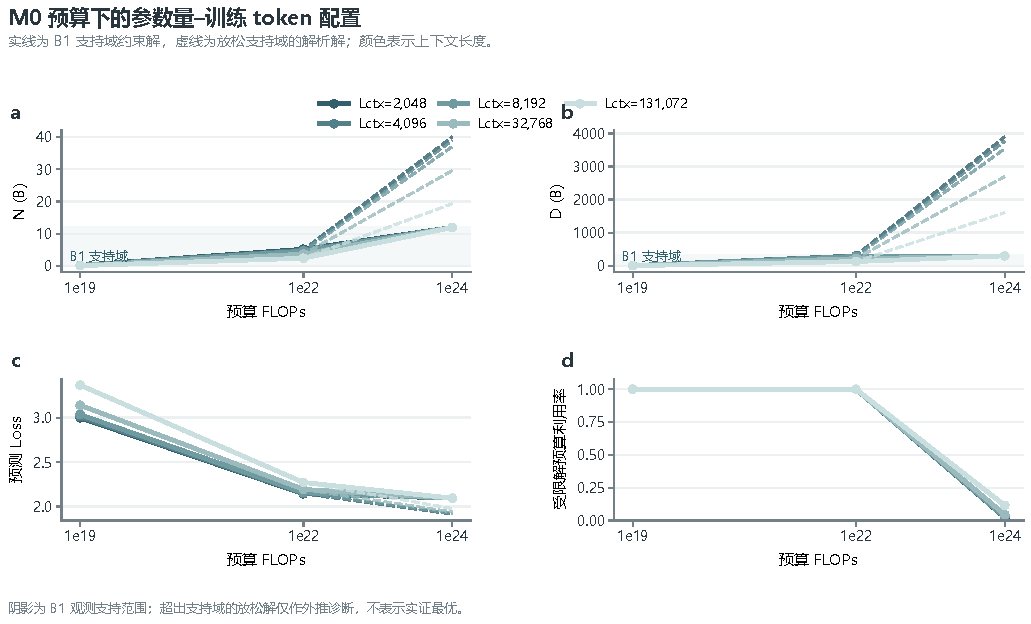
\includegraphics[width=\linewidth]{figures/q3/figures/Fig06_M0_budget_context.pdf}
\caption{M0 预算下的参数量与训练 token 配置。实线为 B1 支持域约束解，虚线为放松支持域的解析解；颜色表示上下文长度。阴影表示 B1 的参数量和 token 支持范围。超出支持域的放松解仅作外推诊断。}
\label{fig:q3-m0-budget}
\end{figure}

\subsubsection{质量投入改变低预算下的资源构成}

M1 的质量投入在低预算下明显依赖成本函数（图~\ref{fig:q3-m1-quality}）。在 $L_{\mathrm{ctx}}=2048$、$C=10^{19}$ FLOPs 时，指数成本得到 $Q^*=0.6985$、$N^*=0.3461$ 和 $D^*=3.4956$，质量成本占总成本约 $22.46\%$；幂函数成本得到 $Q^*=0.5742$，质量成本占比约 $20.24\%$；对数成本直接到达 $Q^*=1$，但把更多预算用于质量处理后，$N^*=0.5763$、$D^*=1.4078$，预测 Loss 为 $3.3146$。因此，质量投入的方向和幅度不能脱离成本函数解释。

预算增加后，三种成本族在 $10^{22}$ FLOPs 及以上的多数情景均到达质量上界。该结果是支持域内的条件最优状态，不能说明真实训练质量一定应达到 1.0。图~\ref{fig:q3-m1-quality} 同时显示，质量成本占比随预算增加而下降，说明规模项重新占据预算主体；这种转移来自当前目标函数和成本假设，而非新增训练观测。

\begin{figure}[htbp]
\centering
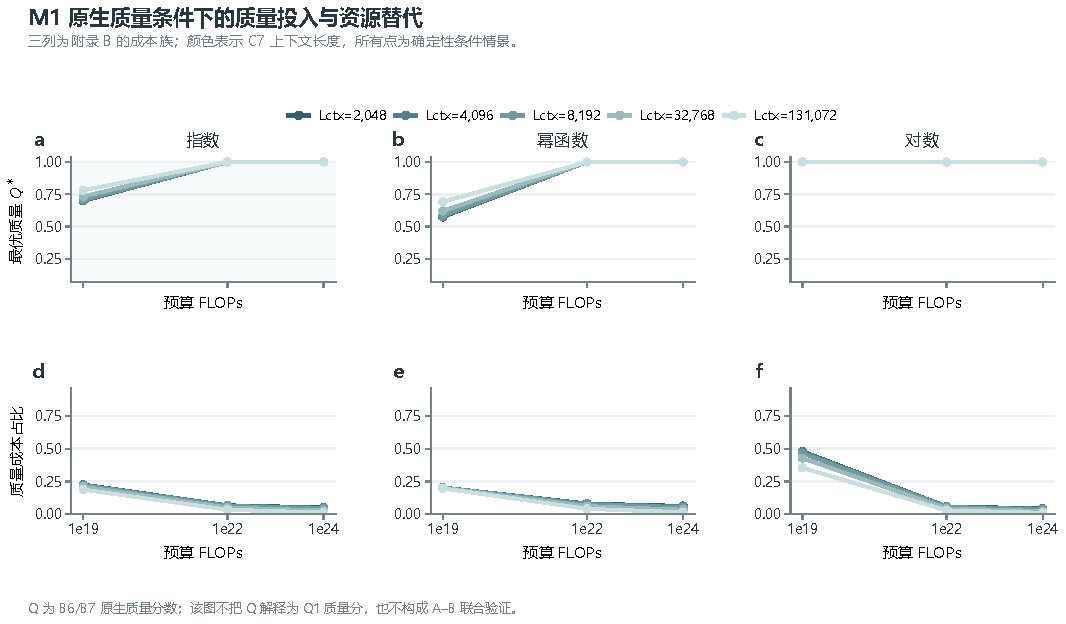
\includegraphics[width=\linewidth]{figures/q3/figures/Fig07_M1_quality_tradeoff.pdf}
\caption{M1 原生质量条件下的质量投入与资源替代。三列分别为指数、幂函数和对数成本；颜色表示 C7 上下文长度。上排为最优质量，下排为质量成本占比。$Q$ 为 B6/B7 原生质量分数，不等同于 Q1 质量分。}
\label{fig:q3-m1-quality}
\end{figure}

\subsubsection{质量结论对初始质量和成本族的敏感性}

为检查质量上界是否由单一初始条件造成，进一步扫描 $Q_0\in\{0.1,0.3,0.5\}$、三类成本函数、五个上下文和三个预算（图~\ref{fig:q3-q0-robustness}）。在 $10^{19}$ FLOPs 下，五个上下文的中位数 $Q^*$ 在指数成本下由 $0.707$（$Q_0=0.1$）降至 $0.687$（$Q_0=0.5$），幂函数成本下由 $0.586$ 降至 $0.531$；对数成本在三个 $Q_0$ 下均到达上界。预算达到 $10^{22}$ FLOPs 后，三种成本族的中位数均为 1.0，并且所有情景到达质量上界。

这一稳健性扫描支持较窄的结论：在本题设成本代理和 B1/B6 支持边界内，低预算的质量选择依赖 $Q_0$ 与成本族，高预算则主要由上界约束决定。它不能替代不同质量处理强度的独立训练实验，也不能证明上界附近的质量提升仍然具有真实 Loss 收益。

\begin{figure}[htbp]
\centering
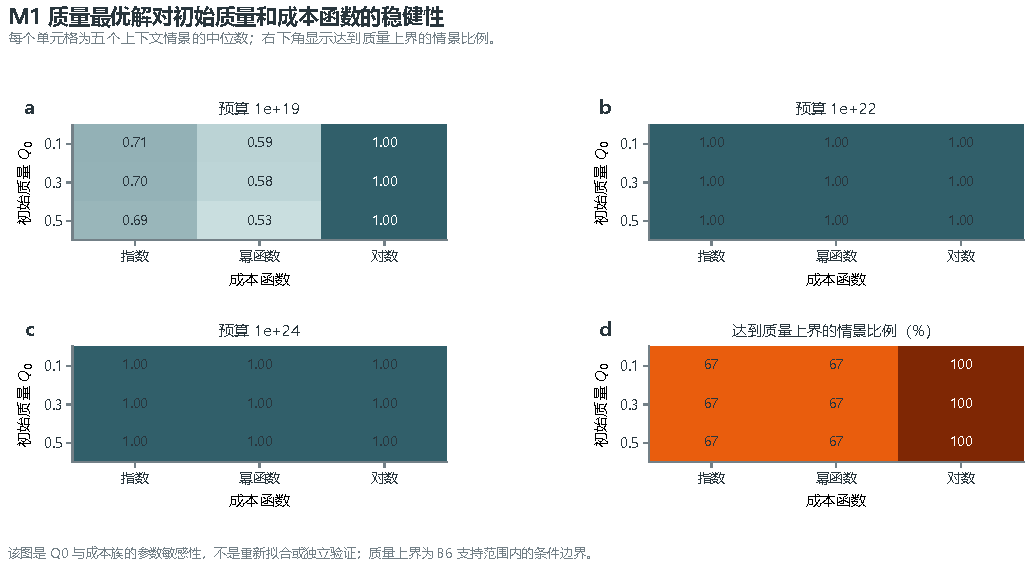
\includegraphics[width=\linewidth]{figures/q3/figures/Fig08_Q0_cost_robustness.pdf}
\caption{M1 质量最优解对初始质量和成本函数的稳健性。每个单元格为五个上下文情景的最优质量中位数；右下角为达到质量上界的情景比例。该图是参数敏感性，不是重新拟合或独立验证。}
\label{fig:q3-q0-robustness}
\end{figure}

\subsubsection{参数折叠传播未改变支持边界这一主导限制}

将 Q2 参数折叠值传播到 Q3 优化器后，M0 在 $10^{19}$ FLOPs 下的 $N^*$ 范围为 $0.1067$--$0.2214$ B、$D^*$ 范围为 $2.9068$--$7.0501$ B tokens；在 $10^{22}$ FLOPs 下分别扩展到 $2.4147$--$5.2024$ B 和 $128.5162$--$299.8930$ B。到 $10^{24}$ FLOPs 时，各上下文的约束解均贴到 B1 的 $N$、$D$ 上界（图~\ref{fig:q3-uncertainty}a,b）。

在指数成本、$L_{\mathrm{ctx}}=2048$ 的 M1 示例中，$10^{19}$ FLOPs 下 $Q^*$ 的折叠传播中位数为 $0.7049$，5\%--95\% 范围为 $0.6831$--$0.7274$；预测 Loss 中位数为 $3.2740$，范围为 $3.2558$--$3.2965$。预算达到 $10^{22}$ FLOPs 后，$Q^*$ 的传播范围收缩到上界，Loss 中位数为 $2.0490$。这些范围是冻结参数的传播结果，而不是独立实验的置信区间。

\begin{figure}[htbp]
\centering
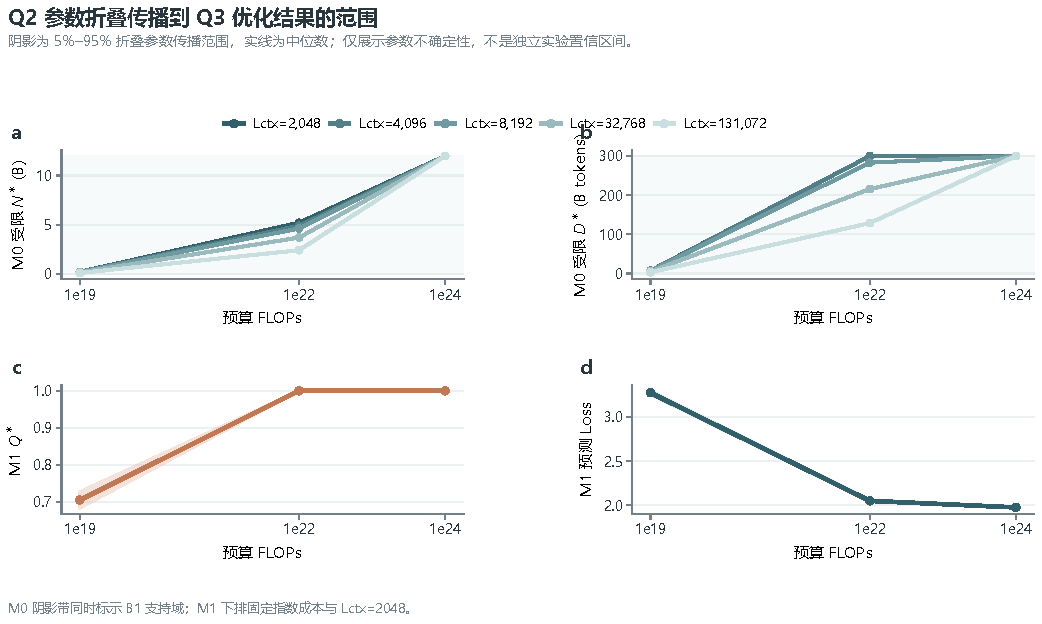
\includegraphics[width=\linewidth]{figures/q3/figures/Fig09_parameter_uncertainty.pdf}
\caption{Q2 参数折叠传播到 Q3 优化结果的范围。阴影为 5\%--95\% 折叠参数传播范围，实线为中位数；仅表示参数不确定性，不是独立实验置信区间。M1 下排固定指数成本和 $L_{\mathrm{ctx}}=2048$。}
\label{fig:q3-uncertainty}
\end{figure}

在固定 $L_{\mathrm{ctx}}=2048$ 的离散成本--Loss 图中，M0 和 M1 的非支配点均来自同一组预算、折叠参数和成本假设（图~\ref{fig:q3-pareto}）。因此，图中的菱形只用于比较已计算情景之间的成本--Loss 关系，不能外推为连续预算下的全局 Pareto 边界。

\begin{figure}[htbp]
\centering
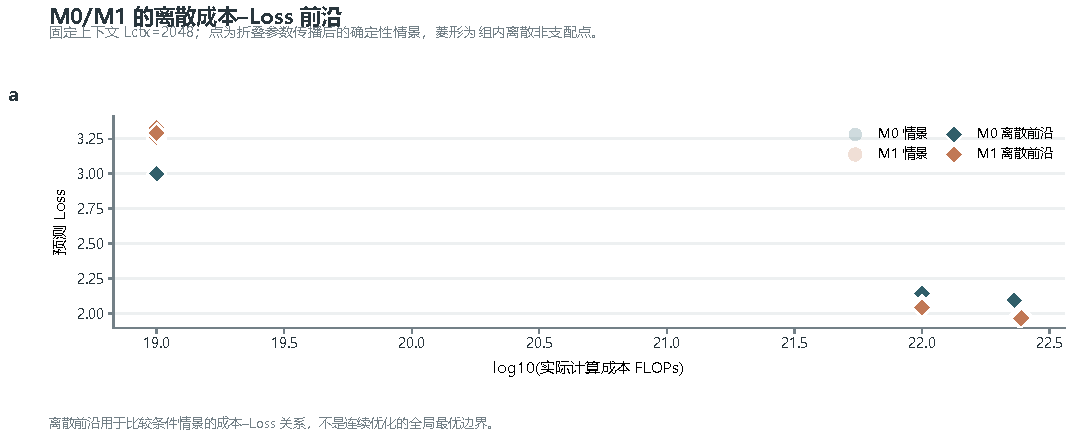
\includegraphics[width=\linewidth]{figures/q3/figures/Fig10_discrete_pareto.pdf}
\caption{M0/M1 的离散成本--Loss 前沿。固定上下文 $L_{\mathrm{ctx}}=2048$；点为折叠参数传播后的确定性情景，菱形为组内离散非支配点。该图不表示连续优化的全局最优边界。}
\label{fig:q3-pareto}
\end{figure}

\subsubsection{已观测配比候选与资源配置需要分开报告}

P 层的六个配比候选在 A 侧的预测排序与观测 scalar Loss 并不完全一致（图~\ref{fig:q3-p-panel}a）。例如，候选 $p46$ 的预测策略排名为 1，但其观测 scalar Loss 为 $-0.7085$；候选 $p170$ 的预测排名为 5，而观测值为 $-0.8268$。这类排序差异说明 A 侧配比预测不能直接当作 B 侧资源配置的验证标签。

在 $L_{\mathrm{ctx}}=2048$、$C=10^{22}$ FLOPs 的 M0 条件配置中，六个候选均得到相同的 $N^*=5.2024$ B、$D^*=299.8930$ B tokens 和预测 Loss $2.1432$（图~\ref{fig:q3-p-panel}b）。这是因为 P 层配比标签没有进入 M0 的 $N,D$ 目标函数，而不是六个配比已经被证明等价。为避免伪造 A--B 联合关系，本文将两侧结果并列展示而不相加。

\begin{figure}[htbp]
\centering
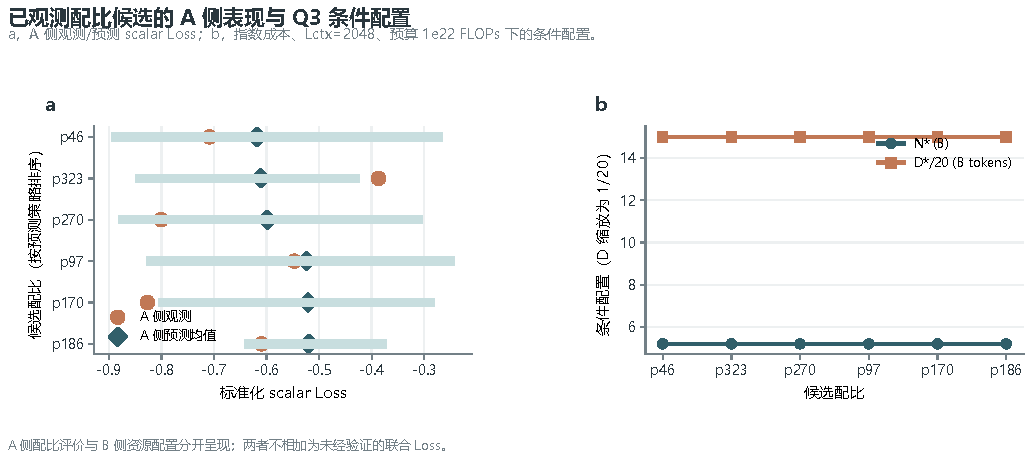
\includegraphics[width=\linewidth]{figures/q3/figures/Fig11_p_candidate_panel.pdf}
\caption{已观测配比候选的 A 侧表现与 Q3 条件配置。a，A 侧观测/预测 scalar Loss；b，指数成本、$L_{\mathrm{ctx}}=2048$、预算 $10^{22}$ FLOPs 下的条件配置。A 侧配比评价与 B 侧资源配置分开呈现，不相加为未经验证的联合 Loss。}
\label{fig:q3-p-panel}
\end{figure}

\subsubsection{Q1 到 B6 的质量接口会改变条件解，但尚未校准}

在指数成本、$L_{\mathrm{ctx}}=2048$、$C=10^{22}$ FLOPs 的固定切片中，五种 Q1--B6 接口情景使假设 $Q_B$ 在候选和映射之间发生明显变化（图~\ref{fig:q3-m2-interface}）。以候选 $p46$ 为例，部分映射原值给出 $Q_B=0.100$、预测 Loss $2.414$；区间高值给出 $Q_B=0.866$、预测 Loss $2.139$，质量成本占比分别为 $0$ 和 $3.2\%$。候选 $p186$ 的同一范围为 $Q_B=0.100$--$0.965$，预测 Loss 为 $2.414$--$2.106$，质量成本占比最高达到 $5.5\%$。

这些差异是接口假设的敏感性，而不是 Q1 分数与 B6 分数已经建立了经验等价。当前数据没有共同批次的质量测量，也没有 $G_{\mathrm{bridge}}$ 的可估计连接项，因此 M2 只能作为反事实接口分析，不能选出跨来源的唯一最优配比。

\begin{figure}[htbp]
\centering
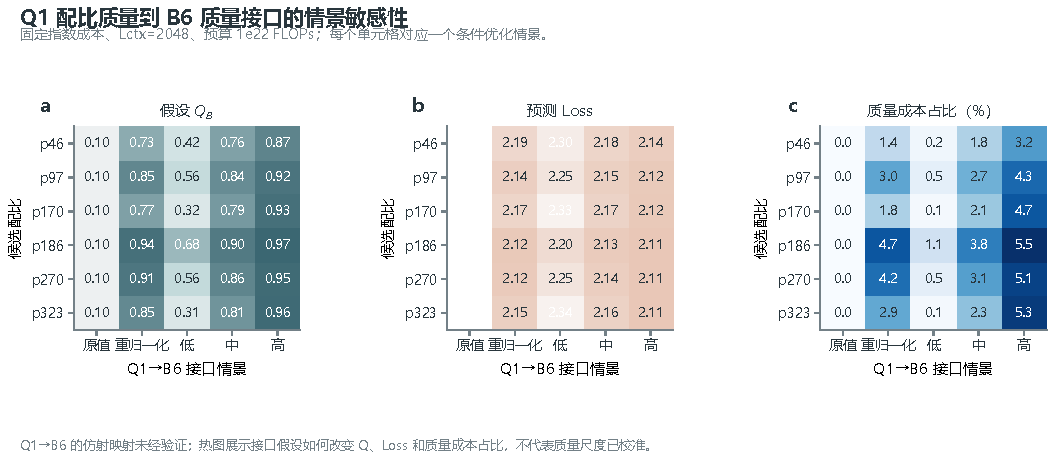
\includegraphics[width=\linewidth]{figures/q3/figures/Fig12_M2_interface_heatmap.pdf}
\caption{Q1 配比质量到 B6 质量接口的情景敏感性。固定指数成本、$L_{\mathrm{ctx}}=2048$ 和预算 $10^{22}$ FLOPs；每个单元格对应一个条件优化情景。Q1 到 B6 的映射未经验证，热图不代表质量尺度已校准。}
\label{fig:q3-m2-interface}
\end{figure}

\subsection{讨论与结论边界}

问题三的主要结果是一个分层的资源配置诊断。M0 说明 B1 支持域内可以计算 $N,D$ 的预算分配，但高预算情景会被支持边界截断；M1 说明原生 B6 质量条件下，低预算质量投入受成本函数和初始质量影响，高预算解容易到达质量上界；P/M2 说明配比候选和跨尺度质量接口会改变条件情景的数值，却不能在缺少连接键时提供联合因果解释。

为明确这些结论的适用范围，图~\ref{fig:q3-identifiability} 将数据块、可计算路径和阻断路径并列表示。当前不能把 A 侧配比 Loss、B1 规模 Loss 和 B6 质量效应相加成一个经过独立验证的四量目标；也不能把支持域外的放松解、M2 的假设 $Q_B$ 或 M1 的质量上界写成真实训练建议。下一步需要共同批次的 A--B 连接键、统一的质量标度和预先固定的独立候选集，才能检验 $G_{\mathrm{bridge}}$、跨块交互以及推荐方案的 top-$k$ regret。

\begin{figure}[htbp]
\centering
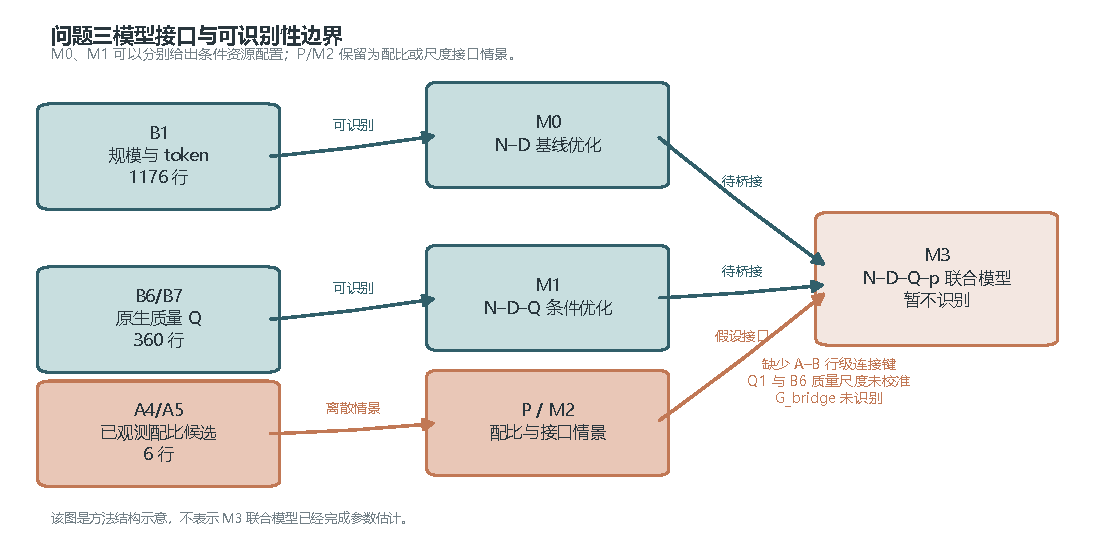
\includegraphics[width=\linewidth]{figures/q3/figures/Fig13_identifiability_interface.pdf}
\caption{问题三模型接口与可识别性边界。M0、M1 和 P/M2 分别给出规模、原生质量和配比接口的条件路径；M3 四量联合模型因缺少 A--B 行级连接键、Q1--B6 质量尺度校准和 $G_{\mathrm{bridge}}$ 而暂不识别。}
\label{fig:q3-identifiability}
\end{figure}

综上，问题三目前支持的是可追溯的条件资源配置和接口敏感性，而不是无条件的四量广义标度律。该边界与数值求解器的复核结果相互独立：求解误差可以很小，并不意味着外推域、成本尺度或跨来源桥接已经得到实证验证。
